\chapter{Introducción}
\label{chapter:introduccion}


%%% SECTION
\section{Descripción general del problema}

% Descripción general del problema~\cite{webscraping}.
En la actualidad, abundan las ofertas de financiación y apoyo económico promovidas por organismos tanto públicos como privados. 
Sin embargo, las organizaciones empresariales encuentran dificultades para determinar qué oportunidades realmente se ajustan a su perfil específico. 
El gran caudal de datos y su heterogeneidad crean un panorama confuso, agravado por la carencia de sistemas automatizados que faciliten una búsqueda eficiente.

Entre las dificultades no solo se encuentra el hallazgo de convocatorias apropiadas, sino también entender la documentación requerida, los cronogramas de presentación, y determinar si estas ayudas son realmente aplicables al contexto empresarial particular. 
Adicionalmente, las compañías deben gestionar información fragmentada y frecuentemente desorganizada distribuida en múltiples fuentes digitales, lo que incrementa la complejidad del proceso de filtrado y selección.

Este proyecto plantea una solución que agilize, simplifique y optimice este proceso de búsqueda de financiación. 
Mediante la combinación de tecnologías como Inteligencia Artificial Generativa \cite{iag}, Procesamiento de Lenguaje Natural (NLP) \cite{Khurana_2022} y métodos de extracción de datos web o scraping \cite{webscraping}, es posible extraer información precisa, relevante y estructurada sobre la documentación de estas convocatorias.

La importancia de esta solución se encuentra en su potencial para reducir tiempos y aumentar la efectividad al elegir opciones de financiamiento adecuadas. 
El hecho de implementar una solución como esta influirá positivamente en las tasas de éxito de las solicitudes presentadas y en la consecución de recursos económicos. 
El propósito de esta solución es democratizar el acceso a oportunidades financieras, fomentando condiciones más favorables para el desarrollo y la continuidad de las empresas.

\newpage

\section{Explicación de la motivación personal}

La motivación tras este proyecto nace del interés personal sobre el uso de las nuevas tecnologías, especialmente la Inteligencia Artificial, en aspectos de la vida, tanto personales como profesionales, donde pueden suponer un cambio importante en la forma de realizar ciertas tareas: Agilizando procesos, reduciendo la dificultad en algunos casos y, en resumen, facilitar y hacer más accesible ciertos aspectos de la vida personal y profesional que pueden resultar tediosos.

El uso de tecnologías como el Procesamiento de Lenguaje Natural y la Inteligencia Artificial Generativa están cambiando desde hace unos años nuestra tecnología a un ritmo nunca visto. Prácticamente cada pocos meses aparecen nuevas tecnologías basadas en este campo de conocimiento, pasando por nuevos Grandes Modelos del Lenguaje como GPT-4o o DeepSeek, nuevas herramientas de desarrollo como Langchain, LLamaIndex, u Ollama, e incluso aplicaciones basadas en IA como Cursor, NotebookLM, o diferentes aplicaciones que te permiten generar texto, imágenes o música sin ser un experto.

Todas estas tecnologías están cambiando la forma en la que vemos el mundo, y aunque es necesario cierto control y regulación para no acabar en unos años en una sociedad distópica digna de la ciencia ficción, sí que considero que tenemos que aprovechar el potencial de estas tecnologías, para seguir el camino, como siempre considero que hay que hacer, hacia una sociedad más justa, equitativa, y donde tenga más peso la calidad de nuestras vidas y los derechos sociales, que las obligaciones económicas y laborales que marcan nuestro día a día.

En este caso concreto del proyecto, el uso de estas técnicas permite democratizar y hacer más accesible este tipo de ayudas. Crear una empresa y mantenerla a flote no es fácil, y en muchos casos sólo unas pocas sobreviven más de unos pocos años tras su creación, generalmente porque parten de unas capacidades económicas por detrás que no disponen el resto. Este tipo de ayudas económicas permiten a empresas con menos recursos de partida salir adelante, y herramientas como estas facilitan la búsqueda y su participación en éstas.

\newpage

\section{Definición de los objetivos}

\subsection{Objetivo Principal}

El objetivo principal de este proyecto es el desarrollo de una solución automática basada en Inteligencia Artificial Generativa, que permita la indexación de información a partir de unas fuentes de datos concretas, en este caso convocatorias de ayudas a empresas, y realice tareas de extracción y estructuración de la información. 
De esta forma, se generará un barrido de todas las posibles convocatorias y se generará una base de datos con información relevante para su consulta y explotación.


\subsection{Objetivos Específicos}

\begin{itemize}

\item \textbf{Implementación de una herramienta de extracción de información}:\\
En primer lugar se diseñará una herramienta que sea capaz de identificar las diferentes convocatorias de ayudas a partir de las fuentes disponibles y extraer la información necesaria:
\begin{itemize}
    \item Codigo fuente de la página web de convocatorias.
    \item Ficha técnica de las convocatorias.
    \item Documentos asociados.
\end{itemize}
Esta herramienta será una combinación de soluciones basadas en Inteligencia Artificial Generativa y Web Scraping.

\item \textbf{Sistema NLP de extracción y procesado de información}:\\ 
Una vez extraída la información de la convocatoria, se emplearán diferentes técnicas de Procesamiento de Lenguaje Natural para diferentes tareas de procesado de texto y extracción de información. 
Este sistema empleará Grandes Modelos del Lenguaje (LLMs) en combinación con diferentes frameworks de orquestación, como Langchain o LLamaIndex.
Se emplearán diferentes propuestas de LLMs para evaluar su eficacia en la extracción de información.

% opcional si da tiempo
\item \textbf{Herramienta de consulta de información}:\\
Finalmente, se implementará una solución de consulta y recuperación de información sobre las diferentes convocatorias, partiendo tanto de los datos estructurados generados en el paso anterior como de las fuentes originales de datos.
Esta solución se basará en un RAG multiagente, empleando técnicas avanzadas en cuanto a Question Answering y procesamiento de texto.
\end{itemize}

\newpage

\section{Descripción de la metodología empleada en el desarrollo del proyecto}





\newpage

\section{Planificación o plan de investigación del proyecto}

Planificación o plan de investigación del proyecto.

% En la actualidad, los procesos de minería de datos requieren grandes cantidades de datos, que en muchas ocasiones contienen información personal y privada de usuarios o personas. Aunque se realicen procesos básicos de anonimización sobre los datos, es decir, eliminación de los nombres u otros identificadores clave, existen multitud de técnicas de re-identificación que permiten volver a identificar a un usuario dentro de este conjunto de datos. En la Figura \ref{fig:context-anoni1} se presenta un mapa donde es posible contextualizar los procesos de anonimización y re-identificación dentro de un proceso de minería de datos.

% \begin{figure}
% 	\centering
% 	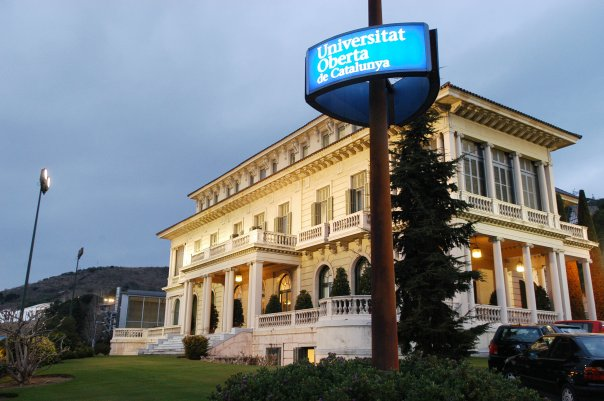
\includegraphics[width=0.6\textwidth]{figs/image1.png}
% 	\caption{Pie de la imagen.}
% 	\label{fig:context-anoni1}
% \end{figure}

% \subsection{Ejemplo de subsection}

% Aunque se han realizado importantes avances en preservación de la privacidad en publicación de datos, tales como el modelo \textit{k}-anonymity \cite{Sweeney:2002}.

% Un ejemplo de pseudo-código se puede encontrar en el Código \ref{code:RandomSwitch-1}

% \begin{algorithm}
% 	\caption{Pseudocódigo del algoritmo \textit{Random Switch}}
% 	\label{code:RandomSwitch-1}
% 	\begin{algorithmic}
% 		\REQUIRE{El grafo original $G$ y el porcentaje de anonimización $p$ que se desea aplicar.}
% 		\ENSURE{El grafo $G$ anonimizado.}
% 		\STATE $num = round(G.num\_edges() * p)$
% 		\STATE $i = 0$
% 		\WHILE {$i < num$}
% 		\STATE {$e_{1} = G.random\_edge()$}
% 		\STATE $e_{2} = G.random\_edge()$
% 		\STATE $new\_e_{1} = (e_{1}.origen, e_{2}.origen)$
% 		\STATE $new\_e_{2} = (e_{1}.destino, e_{2}.destino)$
% 		\IF {$!G.exist(new\_e_{1})$ \AND $!G.exist(new\_e_{2})$}
% 		\STATE $G.add\_edge(new\_e_{1})$
% 		\STATE $G.add\_edge(new\_e_{2})$
% 		\STATE $G.delete\_edge(e_{1})$
% 		\STATE $G.delete\_edge(e_{2})$
% 		\STATE $i=i+1$
% 		\ENDIF
% 		\ENDWHILE
% 		\RETURN $G$
% 	\end{algorithmic}
% \end{algorithm}

% Un ejemplo de tabla se puede ver en la Tabla \ref{table:ejemplo_vertex_refi_query}

% \begin{table}
% 	\centering{}
% 	\begin{tabular}{ l || c | c | l }
% 		\hline
% 		Node ID & $\mathcal{H}_{0}$ & $\mathcal{H}_{1}$ & $\mathcal{H}_{2}$ \\
% 		\hline
% 		\hline
% 		Alice & $\epsilon$ & 1 & \{4\}  \\
% 		\hline
% 		Bob & $\epsilon$ & 4 & \{1, 1, 4, 4\}  \\
% 		\hline
% 		Carol & $\epsilon$ & 1 & \{4\}  \\
% 		\hline
% 		Dave & $\epsilon$ & 4 & \{2, 4, 4, 4\}  \\
% 		\hline
% 		Ed & $\epsilon$ & 4 & \{2, 4, 4, 4\}  \\
% 		\hline
% 		Fred & $\epsilon$ & 2 & \{4, 4\}  \\
% 		\hline
% 		Greg & $\epsilon$ & 4 & \{2, 2, 4, 4\}  \\
% 		\hline
% 		Harry & $\epsilon$ & 2 & \{4, 4\}  \\
% 		\hline
% 	\end{tabular}
% 	\caption{\textit{Vertex refinement queries}.}
% 	\label{table:ejemplo_vertex_refi_query}
% \end{table}





% \section{Introducción v2}

% Esta plantilla pretende ser una guía para los estudiantes. Esta plantilla se puede adaptar a las necesidades específicas de cada proyecto si el supervisor del proyecto está de acuerdo con los cambios.

% \begin{figure}[h]
% \centering
% 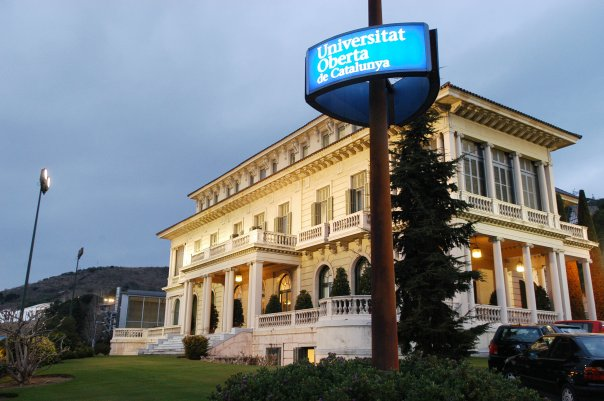
\includegraphics[width=0.5\textwidth]{./figs/image1.png}
% \caption{Ejemplo de figura. Será indexada en la “Lista de Figuras”.}
% \label{fig:figura_ejemplo}
% \end{figure}

% \subsection{Contexto y motivación}

% Punto de partida del proyecto (¿Cuál es el problema que necesita ser resuelto? ¿Por qué es un tema relevante? ¿Cómo se está resolviendo el problema actualmente?) y descripción de la contribución (¿Qué resultado se espera obtener?)

% \subsection{Objetivos}

% Listado de los objetivos a alcanzar en este proyecto.

% \subsection{Sostenibilidad, diversidad y desafíos ético/sociales}

% Esta sección debe evaluar el impacto positivo/negativo del proyecto en las siguientes dimensiones. No es necesario alcanzar un impacto positivo en todas las dimensiones, pero es necesario considerar y discutir si existe un impacto desde el inicio del proyecto.

% \begin{description}
%     \item[Sostenibilidad] En el desarrollo del proyecto o durante todo su ciclo de vida (por ejemplo, despliegue, retiro), ¿tiene el resultado de este proyecto un impacto en la sostenibilidad y/o huella ecológica (consumo/ahorro de energía/recursos, desperdicio, contaminación, agotamiento de materias primas)? ¿Está afectado por leyes o regulaciones sobre este asunto? Considerando otra perspectiva, ¿afecta a alguno de los Objetivos de Desarrollo Sostenible (ODS) relacionados con estas dimensiones? Si no tiene ningún impacto, ya sea positivo o negativo, debe explicar cómo llegó a esta conclusión y justificar su respuesta.
%     \item[Comportamiento ético y responsabilidad social] ¿Es el resultado del proyecto demasiado técnico para tener algún impacto positivo/negativo en aspectos éticos/sociales? ¿Tiene un impacto en leyes/regulaciones (datos, privacidad, trabajo, propiedad intelectual, seguridad personal, …)? ¿Se adhiere a los principios deontológicos de la profesión? ¿Pone en peligro/mejora/empeora algún puesto de trabajo? Si no tiene ningún impacto, ya sea positivo o negativo, debe explicar cómo llegó a esta conclusión y justificar su respuesta.
%     \item[Diversidad, género y derechos humanos] ¿Es el resultado de este proyecto tan técnico que no tiene impacto positivo/negativo en términos de género, diversidad o derechos humanos? ¿Y en leyes/regulaciones? ¿Y en términos de accesibilidad, discapacidad, ergonomía y/o seguridad de la información? Si no tiene ningún impacto, ya sea positivo o negativo, debe explicar cómo llegó a esta conclusión y justificar su respuesta.
% \end{description}

% \subsection{Enfoque y metodología}

% Describa las estrategias potenciales para desarrollar este proyecto y explique la estrategia seleccionada. Discuta por qué la estrategia seleccionada es la más adecuada para alcanzar los objetivos del proyecto.

% \subsection{Planificación}

% Descripción de los recursos necesarios para desarrollar el proyecto, las tareas a realizar y una planificación temporal de cada tarea utilizando un diagrama de Gantt o equivalente. Esta planificación debe definir los hitos que se completarán en cada Prueba de Evaluación Continua (PEC).

% \subsection{Resumen de los productos del proyecto}

% No es necesario describir cada producto en detalle: esto se hará en los capítulos restantes del proyecto.

% \subsection{Breve descripción de los demás capítulos del informe}

% Breve descripción de los contenidos de cada capítulo y su relación con el resto del proyecto.
